\documentclass[11pt]{article}
\usepackage{amsmath, amssymb, amsfonts,  graphicx, enumerate, float, wrapfig, hyperref}
\usepackage[margin=0.5in]{geometry}
\graphicspath{{./}}
\newcommand*{\vs}{\vspace{1cm}}
\newcommand*{\next}{\noindent}
\newcommand*{\set}{\setcounter{equation}{0}}
\newcommand*{\im}{\includegraphics}

\begin{document}

\title{Notes - 4.4 The Fundamental Theorem of Calculus}
\author{Juan J. Moreno Santos}
\date{November 2023}

\maketitle

\begin{enumerate}
    \item Evaluate a definite integral using the Fundamental Theorem of Calculus.
    \item Understand and use the Mean Value Theorem for Integrals.
    \item Find the average value of a function over a closed interval.
    \item Understand and use the Second Fundamental Theorem of Calculus.
    \item Understand and use the Net Change Theorem.
\end{enumerate}

The theorem states that differentiation and (definite) integration are inverse operations.
\begin{enumerate}[(a)]
    \item Differentiation\\ 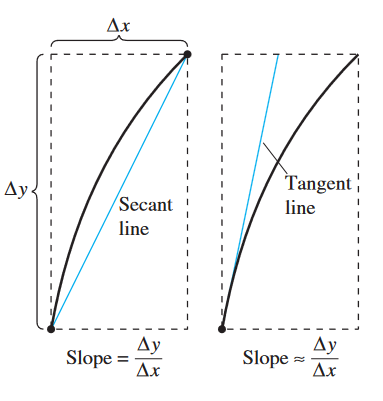
\includegraphics{diff.png}\\
    \item Definite integration\\ 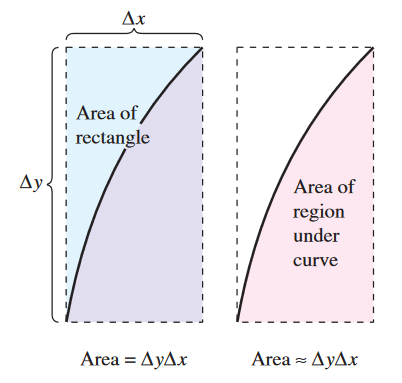
\includegraphics{int.png}
\end{enumerate}

\section{The fundamental theorem of calculus (again)}
If a function $f$ is continuous on the closed interval [a, b] and $F$ is an antiderivative of $f$ on the interval [a, b], then
\[\int_{a}^{b}f(x)dx=F(b)-F(a)\]
In other words, every function that is continuous has an integral

\subsection{Guidelines for using the fundamental theorem of calculus}
\im[scale=0.75]{guidelines.png}

\section{Example - A definite integral involving absolute value}
Evaluate $\int_{0}^{2}|2x-1|dx$.\\
\im[scale=0.75]{ex2.png}
\im[scale=0.6]{ex21.png}

\section{Mean value theorem for integrals}
If $f$ is continuous on the closed interval [a, b], then there exists a number in the closed interval [a, b] such that
\[\int_{a}^{b}f(x)dx=f(c)(b-a)\]
Average height of the function over a certain period of time.\\
\im{proof.png}

\subsection{Average value of a function}
If $f$ is integrable on the closed interval [a, b], then the average value of $f$ on the interval is
\[\frac{1}{b-a}\int_{a}^{b}f(x)dx\]

\section{The second fundamental theorem of calculus}
\im{second.png}\\
\im{ex6.png}\\
If $f$ is continuous on an open interval $I$ containing $a$, then, for every $x$ in the interval,
\[\frac{d}{dx}(F(x)-F(a))=\frac{d}{dx}\left(\int_{a}^{x}f(t)dt\right)=f(x)\]

\section{Net change theorem}
\[\int_{a}^{b}F'(x)dx=F(b)-F(a)\]
\im{ex9.png}\\

\newpage
\im{ex10.png}

\section{11/30/2023 - Warm-up}
1. If $\frac{dy}{dx}=\cos(2x)$, then $y=$
\begin{align}
    \set
    dy&=\cos(2x)dx\\
    &=\int cos(2x)dx\\
\end{align}
Using u-substitution:
\begin{align}
    u&=2x\\
    du&=2dx\\
    \frac{du}{2}&=dx
\end{align}
Therefore, following euqation 3
\begin{align}
    &=\int\frac{1}{2}\cos(u)du\\
    y&=\frac{1}{2}\int\cos udu\\
    &=\frac{1}{2}\int\cos udu+C\\
\end{align}
Substituting back the u:
\begin{align}
    y&=\frac{1}{2}\sin u+C\\
    &=\frac{1}{2}\sin(2x)+C
\end{align}

\vs\next
2. The absolute maximum value of $f(x)=x^3-3x^2+12$ on the closed interval occurs when $x=$
\begin{align}
    \set
    f'(x)&=3x^2-6x=0,\,\, (-2, 4)\\
    &=3x(x-2)=0\\
    3x&=0\,\,\text{and}\,\, x-2=0\\
    x&=0,\,\,2\,\, \text{are critical numbers}
\end{align}
First Derivative Test:
\begin{align}
    f'(0)<12
    f'(4)>12
\end{align}
Therefore, $x=4$ is the absolute maximum.


































































\end{document}